\documentclass[review]{elsarticle}
\usepackage[spanish]{babel}
\usepackage[utf8]{inputenc}
\usepackage{lineno,hyperref}
\modulolinenumbers[5]
\usepackage{mathptmx} % assumes new font selection scheme installed
\usepackage{amsmath} % assumes amsmath package installed
\usepackage{amssymb}  % assumes amsmath package installed

\journal{Journal of \LaTeX\ Templates}
%%%%%%%%%%%%%%%%%%%%%%%
%% Elsevier bibliography styles
%%%%%%%%%%%%%%%%%%%%%%%
%% To change the style, put a % in front of the second line of the current style and
%% remove the % from the second line of the style you would like to use.
%%%%%%%%%%%%%%%%%%%%%%%

%% Numbered
%\bibliographystyle{model1-num-names}

%% Numbered without titles
%\bibliographystyle{model1a-num-names}

%% Harvard
%\bibliographystyle{model2-names.bst}\biboptions{authoryear}

%% Vancouver numbered
%\usepackage{numcompress}\bibliographystyle{model3-num-names}

%% Vancouver name/year
%\usepackage{numcompress}\bibliographystyle{model4-names}\biboptions{authoryear}

%% APA style
%\bibliographystyle{model5-names}\biboptions{authoryear}

%% AMA style
%\usepackage{numcompress}\bibliographystyle{model6-num-names}

%% `Elsevier LaTeX' style

\bibliographystyle{elsarticle-num}
%\documentclass[a4paper,11pt]{article}



\begin{document}

\begin{frontmatter}
\title{PREPARACI\'ON DE SUSPENSIONES E HIDROGELES MAGN\'ETICOS. PROPIEDADES REOL\'OGICAS}


%% Group authors per affiliation:
\author[a]{William Su\'arez}
\ead{wrsuarez@ute.edu.ec}
\address[a]{Afiliaci\'on X1.}


%%%%%%%%%%%%%%%%%%%%%%%%%%%%%%%%%%%%%%%%%%%%%%%%%%%%%%%%%%%%%%%%%%%%%%%%%%%%%%%%

\begin{abstract}
En el presente trabajo se describe la preparaci\'on de suspensiones e hidrogeles magn\'eticos y la medici\'on de sus principales propiedades reol\'ogicas, el trabajo se efectu\'o en el Departamento de F\'isica Aplicada de la Universidad de Granada. Las part\'iculas de magnetita se prepararon mediante la t\'ecnica de coprecipitaci\'on qu\'imica, que consisti\'o en mezclar una soluci\'on de cloruro f\'errico ($Fe Cl_{3} .6 H_{2}O$) y cloruro ferroso ($Fe Cl_{2} .4 H_{2}O$) al 0.1 M con agitaci\'on mec\'anica a una velocidad de 2000 rpm en presencia de nitr\'ogeno. Esta soluci\'on se calent\'o hasta una temperatura de 90 {\ensuremath{{}^\circ}} C, inmediatamente se duplico la velocidad de agitaci\'on y se agreg\'o r\'apidamente una soluci\'on de hidr\'oxido de amonio ($NH_3$) al 10\% en volumen, instant\'aneamente se form\'o un precipitado oscuro que son las nanopart\'iculas de magnetita.
Este precipitado se lav\'o varias veces con agua destilada para remover los iones $C l^{ -}$ y el hidr\'oxido de amonio remanente.

La s\'intesis utilizada es un poco larga y produce aproximadamente entre 4g a 5g de magnetita, una de las falencias de m\'etodo de coprecipitacion es que no permite un buen control del tama\~no de part\'iculas. Posteriormente se a\~nadi\'o alginato y finalmente cloruro de calcio para el proceso de gelaci\'on. La distribuci\'on del tama\~no de part\'iculas se obtuvo con un equipo Zetasizer Nano ZS de la empresa Malvern Instruments. Para la caracterizaci\'on reol\'ogica de las suspensiones de magnetita y magn\'etica con alginato se efectuaron con un re\'ometro HAAKE MARS utilizando una geometr\'ia de doble cono, mientras que la caracterizaci\'on reol\'ogica de los geles se efectu\'o con un re\'ometro Physica Anton Paar MCR300. Las gr\'aficas reom\'etricas obtenidas permiten verificar
el comportamiento magneto reol\'ogico de los geles.

\end{abstract}

\begin{keyword}
S\'intesis \sep magnetita \sep ferrogeles \sep alginato \sep magneto-reometr\'ia)
\end{keyword}

\end{frontmatter}

\section{Introducci\'on}
Los hidrogeles son sistemas formados por cadenas de pol\'imero flexible entrecruzados dentro de un medio acuoso cont\'inuo. Dependiendo de la composici\'on y m\'etodo de preparaci\'on sus propiedades (mec\'anicas, qu\'imicas, grado de biocampativilidad) cubren un amplio espectr\'o, por lo cual, se los puede aplicar en varios campos incluyendo la ingenier\'ia biom\'edica.

Los hidrogeles magn\'eticos se caracterizan por las part\'iculas magn\'eticas que est\'an incrustadas dentro de la matriz del pol\'imero\emph{\cite{ADFM:ADFM201201708}}.
Dichas part\'iculas permiten la detecci\'on y control del hidrogel, sin que sea necesario un cont\'acto, lo cual ha despertado el inter\'es y numerosos estudios se han realizado\emph{\cite{Lopez-Lopez2015},\cite{KIM20124836},\cite{C6NR00224B},\cite{LopezLopez2017110}}.

La investigaci\'on de las propiedades rel\'ogicas de los hidrogeles es un tema en investigaci\'on que presenta varios retos, debidos a los cambios de estructura, p\'erdida de solvente y efecto de paredes deslizantes. Muchos estudios reol\'ogicos de hidrogeles se orientan a: m\'odulo de almacenamiento en estado estable, cin\'etica de gelaci\'on y transici\'on de estado s\'olido-gel.

En el punto de gelaci\'on del hidrogel es de partiular inter\'es, pues la viscoidad de\ cizalla estable tiende al infinito, por lo cual, se lo suele detectar usando varios m\'etodos.


\begin{itemize}
\item Estudio del punto de sobre cruzado (crossover) del m\'odudo de almacenamiento $\left (G^{ \prime }\right )$ y m\'odulo de descarga $\left (G^{ \prime  \prime }\right )$, aunque este m\'etodo solo es v\'alido cuando $G^{ \prime } \left (\omega \right ) =G^{ \prime  \prime } \left (\omega \right )$ para cualquier frecuencia de oscilaci\'on $\omega $.

\item Criterio de Winter Chambon que identifica el punto en el cual $\tan  \delta  =G^{ \prime  \prime }/G^{ \prime }$ independiente de la frecuencia. \end{itemize}

\section{Reolog\'ia}
La Reolog\'ia es una ciencia interdisciplinar cuyo objeto es el estudio de la deformaci\'on y/o caracter\'isticas de flujo de la materia debidas a la acci\'on de fuerzas mec\'anicas externas \cite{9780851864433}.
En los \'ultimos a\~nos se han logrado avances significativos en el bioreolog\'ia, en la reolog\'ia de pol\'imeros y en la reolog\'ia de la suspensi\'on, haciendo que la Reologia sea esencial para la investigaci\'on cient\'ifica en muchas industrias como las de biotecnol\'ogica, pl\'asticos, pinturas, tintas de impresi\'on, detergentes, aceites, etc\cite{Barnes1989}.



La reolog\'ia se centra en el estudio de los materiales que se encuentran entre los extremos cl\'asicos de solidos el\'asticos Hookeanos y liquidos vicosos Newtoneanos, los extremos cl\'asicos se consideran fuera del \'ambito de la reolog\'ia pues son parte la mec\'anica.
En la pr\'actica, la reolog\'ia generalmente se ha limitado al estudio de las relaciones fundamentales (constitutivas), entre la fuerza y la deformaci\'on en los materiales, principalmente los l\'iquidos. Es conveniente recordar algunas relaciones constitutivas.

\section{Comportamiento el\'astico, viscoso y viscoel\'astico}
Desde el punto de vista reol\'ogico, la conducta m\'as elemental de un material corresponde, al comportamiento el\'astico y al viscoso.

\textbf{S\'olido el\'astico:} es un material cuya deformaci\'on s\'olo persiste mientras se mantiene aplicado sobre \'el un esfuerzo de cizalla $\sigma $ (es decir, una fuerza F, por unidad de \'area A, en la direcci\'on tangente a \'esta), que es directamente proporcional a la deformaci\'on transversal y cuya ecuaci\'on constitutiva es\cite{Barnes1989},\cite{1560815795}:
\begin{equation}\sigma  =G \gamma  \label{Lopez 2.33}
\end{equation}
donde G es el m\'odulo de rigidez y $\gamma $ la deformaci\'on.

\textbf{L\'iquido newtoniano:} es un material que se deforma continua e indefinidamente (es decir fluye) cuando es sometido a un esfuerzo, independientemente de cuan peque{\~n}o sea el esfuerzo aplicado, y cuya ecuaci\'on constitutiva es \cite{Barnes1989},\cite{1560815795}:

\begin{equation}\sigma  =\eta  \dot{\gamma } \label{Lopen 2.34}
\end{equation}

donde $\eta $ es una constante de proporcionalidad denominada viscosidad din\'amica y $\dot{\gamma }$ es la velocidad de deformaci\'on.

Sin embargo, tambi\'en existen materiales el\'asticos que no obedecen a la ley de Hooke y exhiben una dependencia no lineal entre fuerza y deformaci\'on; tambi\'en existen fluidos viscosos que no obedecen a la ley de Newton y exhiben una dependencia no lineal entre la fuerza y la velocidad de deformaci\'on. Este tipo de fluidos se conocen con el nombre de fluidos no newtonianos.

\textbf{Materiales viscoel\'asticos}

Entre los comportamientos el\'astico y viscoso existen diversos comportamientos intermedios. El caso m\'as importante para la reolog\'ia
es el relativo a materiales que exhiben propiedades el\'asticas y viscosas simult\'aneamente: son los llamados materiales viscoel\'asticos (es
decir, s\'olidos el\'asticos que durante la deformaci\'on exhiben ciertos aspectos viscosos) o fluidos elasticoviscosos (es decir, fluidos viscosos
que presentan ciertos comportamientos el\'asticos). Los liquidos cuyo comportamiento no puede ser descrito en base de las ecuaciones de Navier-Stokes
son llamados "l\'iquidos no Newtoneanos", y tales l\'iquidos podr\'ian no o no poseer propiedades viscoelasticas\cite{Barnes1989}.

En general el tipo de respuesta de un material depende de la escala de tiempo involucrada en el experimento de acuerdo con Marcus
Reiner, la naturaleza de la respuesta de un material depende del cociente entre el tiempo de relajaci\'on y el tiempo de experimentaci\'on. Este cociente
se llama n\'umero de D\'ebora (De)

\begin{equation}D_{e} =\tau /T \label{BE1.3}
\end{equation}

Donde $T$ es un tiempo caracter\'istico del proceso de deformaci\'on siendo observado y $\tau $ el tiempo caracter\'istico del material. El tiempo $\tau $ es infinito para un s\'olido el\'astico Hookeano y cero para un l\'iquido viscoso Newtoniano.

La caracterizaci\'on local del estado din\'amico y el flujo de un fluido viene dada por el tensor de esfuerzos, y la del estado cinem\'atico
por el tensor de velocidades de deformaci\'on. Sin embargo, el problema se simplifica enormemente si nos limitamos a casos particulares de flujos simples
en los cuales exista una \'unica componente de la velocidad no nula, en una sola direcci\'on. Estos flujos se llaman flujos laminares de cizalla\cite{1560815795}.

Consideremos una superficie plana peque{\~n}a de \'area $ \Delta s$ en un medio deforme como se indica en la Figura \ref{fig:BF1.1} $n_{x}$, $n_{y}$, y $n_{z}$ representan las componentes normales del vector unitario en las direcciones x, y, z, respectivamente. \'Estas definen la orientaci\'on
de $ \Delta s$ en el espacio. Los puntos normales en la direcci\'on del lado +ve de la superficie.

Decimos que el material en el lado + ve de la superficie ejerce una fuerza con componentes $F_{x}^{(n)}  \Delta s$, $F_{y}^{(n)}  \Delta s$, $F_{z}^{(n)}  \Delta s$, en el material en el lado\textit{\ -}ve, siendo asumido impl\'icitamente que el \'area es lo suficientemente peque{\~n}a para las componentes de la tensi\'on $F_{x}^{(n)}$, $F_{y}^{(n)}$, $F_{z}^{(n)}$ sean considerados constantes en la peque{\~n}a superficie $ \Delta s$. Una notaci\'on m\'as conveniente es sustituir \'estas componentes por componentes de esfuerzo $\sigma _{n x}$, $\sigma _{n y}$, $\sigma _{n z}$, el primer \'indice se refiere a la orientaci\'on de la superficie del plano y el segundo a la direcci\'on de la tensi\'on.
La convenci\'on de signos mayormente aceptada es que $\sigma _{z z}$ (y de manera similar con $\sigma _{y y}$ y $\sigma _{x x}$) positivo es una tensi\'on. Componentes $\sigma _{x x}$, $\sigma _{y y}$ y $\sigma _{z z}$ se denominan ``esfuerzos normales''\ y $\sigma _{z x}$, $\sigma _{z y}$, etc. se denominan ``esfuerzo de cizalla''. Puede demostrarse que $\sigma _{x y} =\sigma _{y x}$, $\sigma _{x z} =\sigma _{z x}$, $\sigma _{y z} =\sigma _{z y}$.


\begin{figure}[h!]
\centering
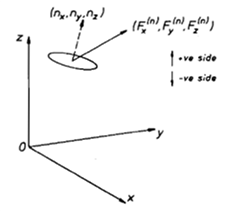
\includegraphics[ width=1.9545in, height=1.7876in,]{./OSAVOB00}
\caption{Los ejes son mutuamente perpendiculares entre s\'i, $0 x$, $0 y$ y $0 z$ y se usan para definir la posici\'on y la orientaci\'on del \'area peque{\~n}a $ \Delta s$ y la fuerza en \'esta.}
\label{fig:BF1.1}
\end{figure}

La Figura \ref{fig:BF1.1} puede ser \'util para explicar la importancia de la notaci\'on indicial. La figura contiene una representaci\'on esquem\'atica de los componentes
del esfuerzo sobre la superficie plana de un peque{\~n}o volumen que forma parte de una cont\'inuo general. Los esfuerzo mostrados son aquellos que act\'uan en el peque{\~n}o volumen debido al material circundante.

\begin{figure}[h!]
\centering
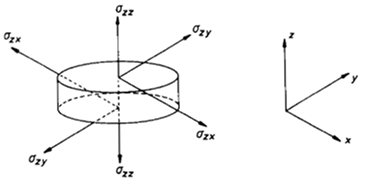
\includegraphics[ width=3.1453in, height=1.5783in,]{./OSAVOB01}
\caption{Los componentes de estr\'es sobre las superficies planas de un elemento de volumen de un medio deformado.}
\label{fig:BE1.2}
\end{figure}


La necesidad de una notaci\'on algebraica es inmediatamente ilustrada por una consideraci\'on m\'as detallada de un flujo
de cizalla simple estable asociado al postulado de Newton Figura \ref{fig:BE1.2} , el cual se puede expresar en la forma
matem\'atica:

$\dot{\gamma } =\frac{v_{x}}{y}$

\begin{equation}v_{x} =\dot{\gamma } y\;\text{,}\;v_{y} =v_{z} =0 \label{BE1.4}
\end{equation}\qquad \qquad \qquad \qquad \qquad \qquad \qquad \qquad

Donde $v_{x}$, $v_{y}$, $v_{z}$ son las componentes de la velocidad en las direcciones x, y y z, respectivamente, $\dot{\gamma }$ es la tasa de cizalla (constate). En el caso de un l\'iquido Newtoniano, la distribuci\'on de la tensi\'on para ese flujo
puede ser escrita en la forma:

\begin{equation}\sigma _{x y} =\eta  \dot{\gamma }\;\text{,}\;\sigma _{x z} =\sigma _{y z} =0\;\text{,}\;\sigma _{x x} -\sigma _{y y} =0\;\text{,}\;\sigma _{y y} -\sigma _{z z} =0 \label{BE1.5}
\end{equation}\qquad \qquad \qquad

Y aqu\'i podr\'ia estar el prop\'osito de considerar cualquier otro que el esfuerzo de cizalla $\sigma _{y x}$ que fue escrito como $\sigma $ en la ecuaci\'on \ref{BE1.1}. N\'otese que es habitual para trabajar en t\'erminos de diferencias de esfuerzo normal lugar esfuerzos normales por s\'i mismos, puesto que estos \'ultimos son arbitrarios a la magnitud de una presi\'on is\'otropa a{\~n}adida en el caso de l\'iquidos incomprensibles, y tendr\'iamos que sustituir (\ref{BE1.5})por

\begin{eqnarray}\sigma _{y x} &  = & \eta  \dot{\gamma }\;\text{,}\;\sigma _{x z} =\sigma _{y z} =0 \label{BE1.6} \\
\sigma _{x x} &  = &  -p\;\text{,}\;\sigma _{y y} = -p\;\text{,}\;\sigma _{z z} = -p \nonumber \end{eqnarray}

Donde p es una presi\'on is\'otropa arbitraria. Est\'a claro que hay m\'erito en el
uso de (\ref{BE1.5}) en lugar de (\ref{BE1.6}) puesto que se evita la necesidad de
introducir p.

Para l\'iquidos el\'asticos, veremos que la distribuci\'on de la tensi\'on es m\'as complicada, nos obliga
a modificar (\ref{BE1.5}) de la siguiente manera:


\begin{eqnarray}\sigma _{y x} &  = & \eta  (\dot{\gamma }) \dot{\gamma }\;\text{,}\;\sigma _{x z} =\sigma _{y z} =0 \label{BE1.7} \\
\sigma _{x x} &  = & N_{1} (\dot{\gamma })\;\text{,}\;\sigma _{y y} = -\sigma _{z z} =N_{2} (\dot{\gamma }) \nonumber \end{eqnarray}

Donde ahora es necesario permitir que la viscosidad var\'ie con la velocidad de cizallamiento,
escrito matem\'aticamente como la funci\'on $\eta  \left (\dot{\gamma }\right )$ y para permitir que las tensiones normales sean distintas de cero y tambi\'en funciones de $\left (\dot{\gamma }\right )$. Aqu\'i el llamado esfuerzo normal diferencias $N_{1}$ y $N_{2}$ son de gran importancia y es dif\'icil ver c\'omo podr\'ian ser convenientemente introducidas sin una notaci\'on algebraica.
Tal notaci\'on es, por lo tanto, no es un extra opcional para los investigadores absolutamente matem\'aticos sino una necesidad absoluta.

\textbf{Viscosidad}

La viscosidad es tradicionalmente considerada como la propiedad m\'as importante de un material
y cualquier estudio pr\'actico que requiera conocimiento de la respuesta material se enfocar\'ia en la viscosidad en primera instancia.

El concepto de viscosidad se introdujo en el numeral 1.2 a trav\'es del postulado de Newton, en el cual el esfuerzo de cizalla $\sigma $ estaba relacionado con el gradiente de velocidad o tasa de cizalla $\dot{\gamma }$, a trav\'es de la ecuaci\'on.

\begin{equation}\sigma  =\eta  \dot{\gamma } \label{BE2.1}
\end{equation}\qquad \qquad \qquad \qquad \qquad \qquad \qquad \qquad \qquad \qquad

Donde $\eta $ es la viscosidad de cizalla. Bajo circunstancias normales la mayor\'ia de ejemplos exhiben caracter\'isticas Newtonianas,
por lo cual $\eta $ es independiente de la tasa de cizalla para la tasa de cizalla de inter\'es.

Para l\'iquidos
Newtonianos, $\eta $ a veces se denomina el coeficiente de viscosidad, ahora es m\'as com\'unmente conocido simplemente como la viscosidad.
Tal terminolog\'ia es \'util dentro del contexto de reolog\'ia, puesto que, en la mayor\'ia de los l\'iquidos, $\eta $ no es un coeficiente sino una funci\'on de la velocidad de cizallamiento $\dot{\gamma }$. Definimos la funci\'on $\eta  \left (\dot{\gamma }\right )$ como la ``viscosidad de cizalla''\ o simplemente viscosidad, aunque en la literatura
esta es\ a menudo referida como la "viscosidad aparente".

Un instrumento concebido para
medir la viscosidad es llamado ``viscos\'imetro''. Un viscos\'imetro es un tipo especial de re\'ometro (definido como un instrumento
para medir las propiedades reol\'ogicas) que se limitan a la medici\'on de viscosidad.

La actual unidad SI de viscosidad es
el Pascal-segundo que se abrevia a Pa.s. Anteriormente, la unidad ampliamente usada de viscosidad en el sistema CGS es el poise, que es m\'as peque{\~n}o
que el Pa.s por un factor de 10.


\section{Resultados preparaci\'on de geles}
Resultados primera preparaci\'on de geles

%Magnetita 5\% vol + 0.10 g Alginato

\begin{table}[h!]
  \centering
  \begin{tabular}{|c|c|c|c|}
  \hline
  Muestra  & $C a C l_{2}$  & Magnetita+Alginato  & Observaciones  \\
  & (ml) & (ml)  &  \\
  \hline
  A & 1.00  & 1.00  & Liquido \\
  \hline
  B  & 1.00  & 0.75 & Liquido  \\
  \hline
  C  & 0.25 & 0.50  & Concentrado  \\
  \hline
  D & 0.50  & 0.25  & Concentrado \\
  \hline
  \end{tabular}
%  \caption{%Magnetita 5\% vol + 0.10 g Alginato}\label{tabla:01}
\end{table}

\section{Conclusiones}
Los objetivos de este trabajo fueron alcanzados, por una parte, se prepararon suspesiones de magnetica e hidrogeles magn\'eticos y por otra se pudieron medir las magnitudes reol\'ogicas que describen el comportamiento materiales magn\'eticos preparados.

El an\'alisis reol\'ogico demostr\'o que el m\'odulo de rigidez, as\'i como los m\'odulos viscoel\'asticos, aumentaron en presencia de nanopart\'iculas magn\'eticas.

Las graficas G' y G''\ versus la amplitud ayudan a deliminart la zona viscole\'astica lineal.

En ambos los ferrogeles y suspensiones con alginato se puedo verificar que las viscosidad se incrementa con en funci\'on del campo magn\'etico aplicado.

\bibliography{mybib}

\end{document}










